\documentclass{estilo}
\usepackage[spanish]{babel}
\usepackage{graphicx}
\usepackage{float}
\usepackage{amsmath}        % para los vectores columnas
\usepackage{amsfonts}       % para las negrita de pizarra
\usepackage{amssymb}        % para simbolos matematicos
\usepackage{hyperref}       % para utilizar referencias
\usepackage{multirow}       % para las tablas
\usepackage{dsfont}
\usepackage{listings}
\usepackage{xcolor}
\definecolor{codegreen}{rgb}{0,0.6,0}
\definecolor{codegray}{rgb}{0.5,0.5,0.5}
\definecolor{codepurple}{rgb}{0.58,0,0.82}
\definecolor{backcolour}{rgb}{0.95,0.95,0.92}
\lstdefinestyle{mystyle}{
    backgroundcolor=\color{backcolour},   
    commentstyle=\color{codegreen},
    keywordstyle=\color{magenta},
    numberstyle=\tiny\color{codegray},
    stringstyle=\color{codepurple},
    basicstyle=\ttfamily\footnotesize,
    breakatwhitespace=false,         
    breaklines=true,                 
    captionpos=b,                    
    keepspaces=true,                 
    numbers=left,                    
    numbersep=5pt,                  
    showspaces=false,                
    showstringspaces=false,
    showtabs=false,                  
    tabsize=2
}
\lstset{style=mystyle}

\usepackage{enumitem,multicol,setspace}
\newcounter{subenum}[enumi] % para las multicolumnas
\renewcommand{\thesubenum}{\arabic{subenum}}
\usepackage[nomessages]{fp}
\FPeval\thecolwidth{round(1/4:4)}% Specify number of columns -> column width
\newcommand{\newitem}[1]{%
  \refstepcounter{subenum}%
  \parbox{\dimexpr\thecolwidth\linewidth-.5\columnsep}{%
    \makebox[\labelwidth][r]{(\thesubenum)\hspace*{\labelsep}}%
    #1}\hfill%
}

\usepackage{scalerel,stackengine} % para el sombrero
\stackMath
\newcommand\rhat[1]{%
\savestack{\tmpbox}{\stretchto{%
  \scaleto{%
    \scalerel*[\widthof{\ensuremath{#1}}]{\kern-.6pt\bigwedge\kern-.6pt}%
    {\rule[-\textheight/2]{1ex}{\textheight}}%WIDTH-LIMITED BIG WEDGE
  }{\textheight}% 
}{0.5ex}}%
\stackon[1pt]{#1}{\tmpbox}%
}
\parskip 1ex

\usepackage{mathtools}      % floor y ceil
\DeclarePairedDelimiter\ceil{\lceil}{\rceil}
\DeclarePairedDelimiter\floor{\lfloor}{\rfloor} 

\usepackage[style=authoryear-comp]{biblatex}

\begin{document}
\newpage
\begin{titlepage}

    \thispagestyle{empty}
    
    \begin{center}
    
\includegraphics[scale=0.3]{imagenes/fiuba.pdf}\\
    \large{\textsc{Universidad de Buenos Aires}}\\
    \large{\textsc{Facultad De Ingeniería}}\\
    \small{Año 2023 - 2\textsuperscript{do} Cuatrimestre}
    \end{center}
    
    \vfill
    
    \begin{center}
    \Large{\underline{\textsc{Análisis Numérico I (75.12 – 95.04)}}}
    \end{center}
    
    \vfill
    
    \begin{tabbing}
    \hspace{2cm}\=\+TRABAJO PRÁCTICO\\
        TEMA:Resolución numérica de problemas de valores iniciales\\
        FECHA:21 de Noviembre 2023\\% \today\\
    \\
        INTEGRANTES:\hspace{-1cm}\=\+\hspace{1cm}\=\hspace{6cm}\=\\
            Aramayo Zambrana, Carolina Luna	\>\> \#106260\\
                \>\footnotesize{$<$caramayo@fi.uba.ar$>$}\\
            Castro Martinez, José Ignacio	\>\> \#106957\\
                \>\footnotesize{$<$jcastrom@fi.uba.ar$>$}\\
            Buchanan, Felix Tomas	\>\> \#102665\\
                \>\footnotesize{$<$fbuchanan@fi.uba.ar$>$}\\
    \end{tabbing}
    
    \vfill
    
    \hrule
    \vspace{0.2cm}
    
    \noindent\small{Análisis Numérico I (75.12 – 95.04) \hfill Catedra Cavaliere}
    
    \end{titlepage}
\newpage
\tableofcontents
\newpage
\newpage
\section{Introducción}
%\flushleft\includegraphics[scale=0.75]{specification.pdf}
Este informe se propone abordar la resoulusión numérica de problemas de valores iniciales a través de los métodos Euler explícito, Euler implícito y Runge Jutta de orden 2. Se quiere resolver un sistema de suspensión vehicualer, el cual se modela como un sistema oscilatorio amortiguador expresado por una ecuación diferencial de segundo grado.
\section{Análisis}
Para empezar, realizamos un análisis del problema de forma física:
\begin{figure}[h] 
    \centering
    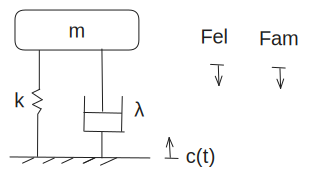
\includegraphics[width=0.5\textwidth]{imagenes/analisis.png}
    \caption{Análisis del caso de estudio}
    \label{fig:figura1}
\end{figure}

\begin{figure}[h] 
    \centering
    \includegraphics[width=0.5\textwidth]{imagenes/circuito.png}
    \caption{Circuito mecanico}
    \label{fig:figura2}
\end{figure}
El enunciado nos da una ecuación diferencial que es la siguiente:
\begin{align}
    y'' &= \frac{k}{m}(c - y) + \frac{\lambda}{m}(c' - y')
\end{align}
Esta representa la aceleración vertical de la carrocería. Es decir, oscilador amortiguado que responde a una excitación dada por la variable c.
\begin{itemize}
    \item \( k \) constante elástica del muelle [N/m]
    \item \( \lambda \) constante de amortiguación [Ns/m]
    \item \( c \) cota o elevación del terreno [m]
    \item \( y \) posición de la carrocería [m]
    \item \( c' \) y \( y' \) son derivadas de \( c \) e \( y \) con respecto al tiempo, es decir, velocidades verticales [m/s]
\end{itemize}
Entonces tenemos a \(c(t)\) y \(y(t)\) por hallar.
Como la solución general se solicita en el punto 1, desarrollaremos los métodos de forma genérica y luego se aplicará en el siguiente punto con lo solicitado.
Para ello debemos discretizar la EDO de segundo orden por los métodos propuestos.
Vamos a discretizar tres parámetros:
\subsection{Discretizar la EDO}
Como es una EDO de segundo orden se debe definir dos nuevas variables
\[
\begin{cases}
    y(t) \approx y(t_n) \approx u_n \\
    y'(t) \approx y'(t_n) \approx u'_n = v_n 
\end{cases}
\]
De esta forma pasamos de una EDO de segundo orden a una EDO lineal
\[
\begin{cases}
    u' = f_1(u,v,t) \\
    v' = f_2(u,v,t)
\end{cases}
\]
\newpage
\section{Desarrollo}
\subsection{Euler explícito}
El método de Euler explícito es de la siguiente manera:
\begin{equation}
u_{n+1} = u_n + h f(u_n, t_n)    
\end{equation}
Para el caso de estudio tenemos:
\[
\begin{cases}
    f_1(u_n,v_n,t_n) = v_n \\
    f_2(u_n,v_n,t_n) = \frac{k}{m}(c - u_n) + \frac{\lambda}{m}(c' - v_n)
\end{cases}
\]
Por lo tanto tenemos las ecuaciones:
\[
\begin{cases}
    u_{n+1} = u_n+hv_n \\
    v_{n+1} = v_n + h [\frac{k}{m}(c - u_n) + \frac{\lambda}{m}(c' - v_n)]
\end{cases}
\]
\textcolor{red}{\textbf{SEGUIR}}
\subsection{Euler implícito}
El método de Euler implícito es de la siguiente manera:
\begin{equation}
u_{n+1} = u_n + h f(u_{n+1}, t_{n+1})
\end{equation}
Para el caso de estudio tenemos:
\[
\begin{cases}
    f_1(u_{n+1},v_{n+1},t_{n+1}) = v_{n+1} \\
    f_2(u_{n+1},v_{n+1},t_{n+1}) = \frac{k}{m}(c - u_{n+1}) + \frac{\lambda}{m}(c' - v_{n+1})
\end{cases}
\]
Por lo tanto tenemos las ecuaciones:
\[
\begin{cases}
    u_{n+1} = u_n+hv_n \\
    v_{n+1} = v_n + h [\frac{k}{m}(c - u_n) + \frac{\lambda}{m}(c' - v_n)]
\end{cases}
\]
\textcolor{red}{\textbf{SEGUIR}}
\subsection{Runge Kutta de orden 2}
El método de RK2 es de la siguiente manera:
$
\begin{cases}
    q_1 = h f(u_n, t_n) \\
    q_2 = h f(u_n + q_1, t_{n+1}) \\
    u_{n+1} = u_n + \frac{1}{2} (q_1 + q_2)    
\end{cases}
$

\textcolor{red}{\textbf{ME TRABÉ AYUDA}}

Para el problema planteamos las ecuaciones:
$
\begin{cases}
    q_1 = hv_n \\
    q_2 = hf(u_n+hv_n,t_{n+1}) \\
    u_{n+1} = u_n + \frac{1}{2} (q_1+q_2)    
\end{cases}
$
\end{document}